%\chapter{Introduction to Linear Programming}
\chapter{Maximum Flow}

\section{Problem Setting}
In this chapter we consider directed graphs and we assign a flow to each arc.
Specifically, given
\begin{enumerate}
\item
A directed graph $G=(N,A)$
\item
A \emph{source node} $s\in N$ and a \emph{sink node} $t\in N$
\item
A function $u:A\to\mathbb{R}^+$, which denotes the \emph{arc capacity}
\end{enumerate}

\begin{definition}[Feasible Flow]
We consider assigning a flow $x_{ij}$ on each arc $(i,j)\in A$ such that
\begin{enumerate}
\item
$0\le x_{ij}\le u_{ij}$
\item
The flow in equals the flow out at each (non-source and non-sink) node.
\end{enumerate}
\end{definition}
We aim to find the maximum amount that can flow from $s$ to $t$.

\section{Linear Programming Formulation}
The maximum flow problem can be formulated using linear programming:
\begin{equation}\label{Eq:6:1}
\begin{array}{ll}
\max&v\\
\mbox{such that}&0\le x_{ij}\le u_{ij},\quad \forall(i,j)\in A\\
&\sum_{(i,j)\in A}x_{ij} - \sum_{(j,k)\in A}x_{jk}=\left\{
\begin{aligned}
-v,&\quad \text{if $j=s$}\\
0,&\quad \text{if $j\in N\setminus\{s,t\}$}\\
v,&\quad\text{if $j=t$}
\end{aligned}
\right.
\end{array}
\end{equation}
Here $v$ is called the \emph{value} of a given flow $x$ from $s$ to $t$.

\subsection{Upper bound on the flow value}
\begin{definition}
$[S,T]$ is called an $s-t$ cut of $G$ if $s\in S,t\in T, S\sqcup T=N$.
\end{definition}

\begin{theorem}
The flow value is upper bounded by the capacity of any cutset $[S,T]$.
\end{theorem}
\begin{proof}
Summing up the second constraint of~(\ref{Eq:6:1}), we imply
\begin{align*}
\sum_{j\in S}&\left[\sum_{(i,j)\in A}x_{ij} - \sum_{(j,k)\in A}x_{jk}\right]=-v\\
\Longleftrightarrow&\sum_{j\in S}\sum_{(i,j)\in A, i\in T}x_{ij}
+
\sum_{j\in S}\sum_{(i,j)\in A, i\in S}x_{ij}
\\&-
\sum_{j\in S}\sum_{(j,k)\in A, k\in S}x_{jk}
-
\sum_{j\in S}\sum_{(j,k)\in A, k\in T}x_{jk}=-v\\
\Longleftrightarrow&\sum_{j\in S}\sum_{(i,j)\in A, i\in T}x_{ij}-\sum_{j\in S}\sum_{(j,k)\in A, k\in T}x_{jk}=-v
\end{align*}
Therefore,
\[
v\le \sum_{j\in S}\sum_{(j,k)\in A, k\in T}x_{jk}\le \sum_{j\in S}\sum_{(j,k)\in A, k\in T}u_{jk},
\]
which is the capacity of the cutset $[S,T]$.
\end{proof}
\begin{corollary}
If for the given feasible flow $x$, the flow value $v_x$ equals $U[S',T']$ for some cutset $[S',T']$, then $v_x$ must be the maximum flow value.
\end{corollary}

\section{Flow Augmentation}
\begin{definition}[Residual Graph]
Given a directed graph $G$ and a feasible $s-t$ flow $x$, we define the corresponding \emph{residual graph} $G_x=(N,A_x)$ with \emph{residual capacities} $r:A\to\mathbb{R}^+$ on the arcs as follows:
\begin{enumerate}
\item
The arc $(i,j)\in A_x$ if 
\begin{itemize}
\item
either $(i,j)\in A$ with $x_{ij}< u_{ij}$
\item
or $(j,i)\in A$ and $x_{ji}>0$
\end{itemize}
\item
The residual capacity of $(i,j)\in A_x$ is $r_{ij} = (u_{ij} - x_{ij}) + x_{ji}$
\end{enumerate}
In other words, the residual graph is such that the residual capacities assigned into each arc is positive, i.e., $G_x = G - x$.
\end{definition}

\begin{definition}[residual capacity of the path]
Let $P_x$ be a directed path from $s$ to $t$ in augmenting network $G_x$.
Define the \emph{residual capacity of the path} $P_x$ as
\[
r(P_x):=\min_{(i,j)\in P_x}r_{ij}
\]
If $r(P_x)>0$, we say that there is an augmenting path from $s$ to $t$.
\end{definition}

Clearly, if $r(P_x)>0$, we can increase the value of the (network) flow by augmenting the flow $x$ with some path in $P_x$.

\begin{theorem}[Optimality condition on maximum flow]
An $s-t$ flow $x$ is of maximum value iff there is no $s-t$ augmenting path w.r.t. $x$.
\end{theorem}
\begin{proof}
For the forward direction, if there is an augmenting path, then clearly flow can be increased.

For the reverse direction, suppose there is no augmenting path w.r.t. x.
Let $S$ be the set of nodes to which there is an augmenting path from $s$, and therefore $t\notin S$.
Let $T=N\setminus S$, which implies
\[
\sum_{i\in S}\sum_{j\in T, (i,j)\in A}
=\sum_{i\in S}\sum_{j\in T, (i,j)\in A}u_{ij},\quad
\sum_{i\in T}\sum_{j\in S, (i,j)\in A}x_{ij}=0
\]
Therefore, $v_x=U[S,T]$, and $v_x$ must be the maximum flow value.
\end{proof}


\begin{algorithm}[htb] 
\caption{Ford-Fulkerson Max-Flow Algorithm} 
\label{alg:SM} 
\begin{algorithmic}[1] %show number in each rows
\STATE If no $s$-$t$ augmenting path exists, then current flow is maximum
\STATE
Otherwise, augment flow (up to residual capacity of augmenting
path); repeat from step~(1)
\end{algorithmic}
\end{algorithm}
\begin{corollary}
If all arc capacities are integer-valued, then the maximum flow value is also integer-valued, so are the arc flows.
\end{corollary}
\begin{proof}
Start with flow value $v_x=0$.
Every flow augmentation increases the flow values by an integer value.
\end{proof}

\paragraph{Efficiency of the Max-Flow Algorithm}
Consider the following max-flow problem:
\begin{figure}[H]
\centering
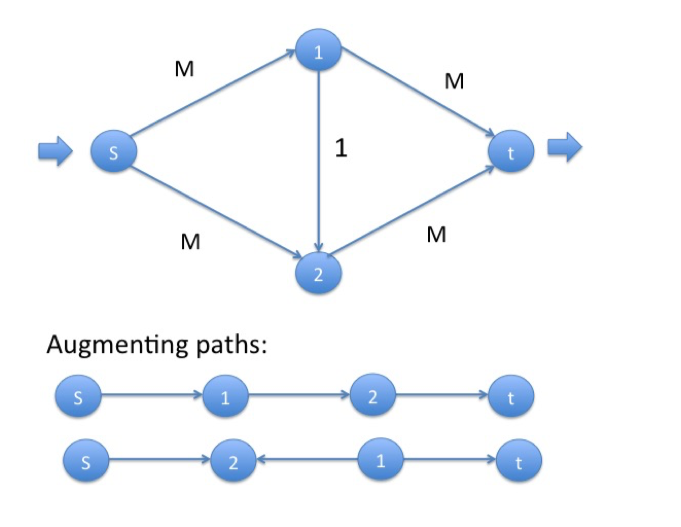
\includegraphics[width=0.7\textwidth]{Sixth_lecture/p_1}
\end{figure}
Each time, we augment by one unit of flow. So it take $2M$ augmentations, which is not efficient.

Therefore, we need the flow decomposition technique.

\section{Flow Decomposition}
Given an assignment of flows $x_{ij}$ to each $(i,j)\in A$, the excess flow at any $j\in A$ is the quantity
\[
e(j) = \sum_{(i,j)\in A}x_{ij} - \sum_{(j,k)\in A}x_{jk}
\]
which denotes the difference between the flow getting into $j$ and the flow getting out of $j$.
If $x$ is a feasible flow, then the excess flow $e(j)$ is always zero, except $j=s,t$.

If $e(j)>0$, then we say $j$ is an \emph{excess} node; if $e(j)<0$, then $j$ is a \emph{deficit} node.
\begin{algorithm}[htb] 
\caption{Flow Decomposition Algorithm} 
\label{alg:SM} 
\begin{algorithmic}[1] %show number in each rows
\STATE 
Start with a node $i_0$ with $e(i_0)<0$ or where there is an arc $(i_0,i_1)$ with positive flow.
Let $k=1$
\STATE
If $i_k$ has $e(i_k)>0$, then we identified a path $P=\{i_0,\dots,i_k\}$.
Set $f(P) = \min\{-e(i_0),e(i_k),\min\{x_{ij}\mid (i,j)\in P\}\}$.
Repeat from step $1$.
\STATE
If $i_k = i_h$ for some $0\le h<k$, then we identified a cycle $W=\{(i_h,i_{h+1}),\dots,(i_{k-1},i_k)\}$.
Set the cycle flow $g(W)=\min\{x_{ij}\mid (i,j)\in W\}$.
Repeat from step $1$.
\item
Otherwise there is an arc $(i_k,i_{k+1})$ with positive arc flow.
Increase $k$ by 1.
Repeat from Step 2.
\end{algorithmic}
\end{algorithm}

Therefore, we decomposed arc-flows into path-flows and cycle-flows.


\begin{theorem}
If flow augmentation is done along an augmenting path of maximum residual capacity of maximum residual capacity, then no more than $P(m\log U)$ augmentations are required to obtain the maximum flow.
\end{theorem}

\begin{theorem}
If flow augmentation is done along an augmenting path with a minimum number of arcs, then no more than $O(mn/2)$ augmentations are required to obtain the maximum flow
\end{theorem}

\section{Dinic’s Algorithm}
\begin{definition}[Level Graph]
Given an augmenting network $G_x$, define the \emph{level} of a node $i$, $\ell(i)$, as the number of arcs in a \emph{shortest} path from $s$ to $i$.

We define the \emph{level graph} $\mathcal{L}_x$ as the subgraph of $G_x$ such that
\begin{itemize}
\item
it contains nodes reachable from $s$
\item
it contains arcs $(i,j)$ such taht $\ell(j) = \ell(i)+1$
\end{itemize}
\end{definition}

\begin{algorithm}[htb] 
\caption{Dinic's Algorithm} 
\label{alg:SM} 
\begin{algorithmic}[1] %show number in each rows
\STATE 
Initially $x=0$.
\STATE
Construct level graph $\mathcal{L}_x$.
\STATE
If $\mathcal{L}_x$ does not contain an $s$-$t$ augment path, stop.
\item
Otherwise, repeat:
\begin{itemize}
\item
find an $s$-$t$ augmenting path $P_x$ in $\mathcal{L}_x$ by depth-first search
\item
augment flow by $r(P_x)$
\end{itemize}
Unitl all $s$-$t$ paths in $\mathcal{L}_x$ have zero residual capacity
\STATE Go to step $2$.
\end{algorithmic}
\end{algorithm}

Using Dinic’s algorithm, the max-flow can be found in $O(n^2m)$ time

\section{Maximum Flow $\&$ Minimum Cut}
\begin{theorem}
For any network, the maximum flow value from source $s$ to sink $t$ is equal to the minimum cut capacity of an $s$-$t$ cut.
\end{theorem}

\begin{definition}[Disconnecting Set]
A $st$-disconnecting set of a graph $G$ is the set of edges $F$ of $G$ such that every path from $s$ to $t$ includes an edge of $F$
\end{definition}

\begin{theorem}[Menger's Theorem~(edge form)]
The maximum number of edge-disjoint paths connecting two distinct vertices $s$ and $t$ of a connected graph is equal to the minimum number of edges in an st-disconnecting set.
\end{theorem}
\begin{theorem}[Menger's Theorem~(vertex form)]
The maximum number of vertex-disjoint paths connecting two distinct non-adjacent vertices $s$ and $t$ of a connected graph is equal to the minimum number of vertices in an $st$-separating set.
\end{theorem}

\begin{theorem}
A graph $G$ is $k$-edge-connected if and only if any two distinct vertices of $G$ are joined by at least $k$ edge-disjoint paths.
\end{theorem}

\begin{theorem}
A graph $G$ with at least $k + 1$ vertices is $k$-connected if and only if any two distinct vertices of $G$ are joined by at least $k$ vertex-disjoint paths.
\end{theorem}

\subsection{System of distict representatives}
Consider a scheduling problem:
\[
S_1=\{3,5,6\},\quad
S_2=\{3,4,6\},\quad
S_3=\{5,8\},\dots
\]
where $S_i$ is the possible time slots for exam $i$.
We want to find a schedule where all the exams are scheduled and no two exams are scheduled at the same time slot.
\begin{definition}[SDR]
In general, we consider
\begin{itemize}
\item
a set of elements $E=\{e_1,\dots,e_m\}$
\item
a collection $\mathcal{S}$ of subsets of $E$: $\mathcal{S}=\{S_1,\dots,S_n\}$
\end{itemize}
We say there is a \emph{system of distinct representatives (SDR)} of $\mathcal{S}$ if there are distinct elements $\{e_{r(1)},\dots,e_{r(n)}\}$ such that $e_{r(i)}\in S_i$ for $i=1,\dots,n$.
\end{definition}

Actually, we can find a SDR by solving a max-flow problem:
We model a graph with vertex $s$, a sink vertex $t$, vertices $E$, and vertices $\mathcal{S}$, and arcs:
\begin{itemize}
\item
$(s,e_i)$ with capacity $1$ for $j=1,\dots,m$
\item
$(S_j,t)$ with capacity $1$ for $j=1,\dots,n$
\item
$(e_i,S_j)$ with infinite capacity if $e_i\in S_j$.
\end{itemize}
If the max $s$-$t$ flow of this network has value $n$, then a SDR exists.
\begin{theorem}[Hall, 1935]
The colletion $\mathcal{S}$ has a SDR if and only if for all $k=1,\dots,n$,
the union of any $k$ sets of $\mathcal{S}$ contain at least $k$ distinct elements.
\end{theorem}
\subsubsection{Applications of SDR}
\begin{theorem}
For a zero-one matrix, the minimum number of \emph{lines} that cover all the $1$'s in the matrix is equal to the maximum number of $1$'s that can be selected such that no two are on the same line.

A line can be either a column or a row.
\end{theorem}
\begin{proof}
Let $\ell$ be the minimum of lines needed, and $L$ be the maximum number of $1$'s selected.
It's clear that $\ell\ge L$. It suffices to show the equality.

Suppose that $\ell=r+c$, i.e., all the $1$'s of the matrix are covered by $r$ rows and $c$ columns (why?).
w.l.o.g.,the rows and columns needed are the top $r$ rows and left-most $c$ columns.

Consider a SDR problem with $\mathcal{S}=\{S_1,\dots,S_r\}$, where $S_i=\{j\mid j>c,a_{ij}=1\}$.
\begin{itemize}
\item
Every union of $k$ sets of $\mathcal{S}$ contain at least $k$ distinct elements:
Suppose on the contrary that $|S_1\cup S_2\cup\cdots\cup S_k|\le k-1$, then all the $1$'s in the first $k$ rows are in $k-1$ columns, then we can cover all the $1$'s in the matrix using $r-k$ rows and $c+(k-1)$ columns, which contradicts to the minimality of $\ell$.
\end{itemize}
Therefore, $\mathcal{S}$ has a SDR.
There exists $r$ 1's in the first $r$ rows and to the right of the first $c$ columns, and no two of which are in the same column.

Similarly, there are $c$ 1's in the first $c$ columns and below the top $r$ rows, and no two of which are in the same row.

Therefore, $L\ge r+c=\ell$.
\end{proof}



\begin{definition}[Latin Square]
A $n$ by $n$ matrix is a \emph{Latin square} if the entries are drawn from a set of $n$ elements such that each element appears exactly once in each row and each column.
\end{definition}
\begin{definition}[Latin Rectangle]
An $r$ by n matrix is an $r$ by $n$ Latin Rectangle if each row contain the numbers $\{1,\dots,n\}$ (in some permutation) and each column does not contain any repeated number.
\end{definition}
\begin{theorem}
Given a Latin rectangle with $r<n$, we can add a row to form an $(r+1)$ by $n$ rectangle.
\end{theorem}

\begin{proof}
Let $S_j, j=1,\dots,n$ be the set of numbers that don't appear in the column $j$.
The SDR for this collection of $n$ sets will be the elements in the row $(r+1)$.

We claim that every $k$ sets in $\mathcal{S}=\{S_1,\dots,S_n\}$ must contain at least $k$ distinct numbers.
Note that the $k$ sets contain $k(n-r)$ numbers counting repeats.

Note that each number can appear in the $k$ sets at most $(n-r)$ times.
Therefore, there must be $k$ distinct numbers in the $k$ sets.

Therefore, by Hall's theorem, there is a SDR and row $(r+1)$ can be added to the Latin Rectangle.
\end{proof}


\subsection{Max-flow Min-cut and Linear Programming Duality}
Consider the circulation model of the max-flow problem, i.e., we introduce the arc $(t,s)$ with infinite capacity.
In this case, we have
\[
\begin{array}{ll}
\max&x_{ts}\\
\mbox{such that}&0\le x_{ij}\le u_{ij},\ \forall(i,j)\in A\\
&\sum_{(i,j)\in A}x_{ij} - \sum_{(j,k)\in A}x_{jk}=0,\ \forall j\in 
\end{array}
\]
The dual problem is given by:
\[
\begin{array}{ll}
\min&\sum_{(i,j)\in A}u_{ij}z_{ij}\\
\mbox{such that}&y_j - y_i + z_{ij}\ge0,\ \forall(i,j)\in A\\
&y_s - y_t\ge1,\ \text{for $(t,s)$}\\
&z_{ij}\ge0, \ \forall(i,j)\in A\\
& y_j\text{unrestricted in sign}, \forall j\in N
\end{array}
\]
Consider a feasible solution defined by an $s$-$t$ cut $[S,T]$:
\[
y_j=\left\{
\begin{aligned}
1,&\quad j\in S\\
0,&\quad j\in T
\end{aligned}
\right.
\qquad
z_{ij}=\left\{
\begin{aligned}
1,&\quad\text{if $(i,j)\in A,i\in S,j\in T$}\\
0,&\quad\text{otherwise}
\end{aligned}
\right.
\]
The objective value is 
\[
\sum_{(i,j)\in A, i\in S,j\in T}u_{ij}=U[S,T],
\]
which is the capacity of the cut.


We can also show the max-flow min-cut theorem using linear programming duality.















